
\section{Basic Models}
I want to create some basic models in this section to help me visualize the problem; it can also test my conjuncture of the continuous approximations.

%Firstly, I wish to find an optimal starting condition --- this leads to the precalculation of the vertical motion. Secondly, I will model the motion of the remaining two axis of motion. Lastly, I will fit various acceleration models using my experience, some calculus, and even polar coordinates.

% straight line
\subsection{Key idea and boundary conditions}
The key idea that will be repeated throughout models is that the maximization of the player velocity and acceleration will maximize the jump displacement. I hypothesized this from the positional differential equations, Eq. \ref{eq:1de2}, where if velocity is constant, the final displacement will be proportional to that constant:
\begin{align*}
    \tp'(t) &= \tv(t)\\
    \tp(t) &= \int \tv(t) \, dt\\
    &= t\tv(t) + \tp(0) = t\tv(t) + \tzero,\\
    \tp &\propto \tv(t).
\end{align*}

Using this idea, I devised an optimal initial velocity for the player --- the boundary condition of the problem. For we are maximizing the jump displacement, and higher velocity equates to higher displacement, it is reasonable to set the initial velocity/speed as high as possible. So
\[
    \tmag{\tv(0)} = 250,
\]
where $250$ is fastest ground running speed\citefoot{counter_2022}.


\begin{figure}[H]
    \centering
    \begin{minipage}{.5\textwidth}
        \centering
        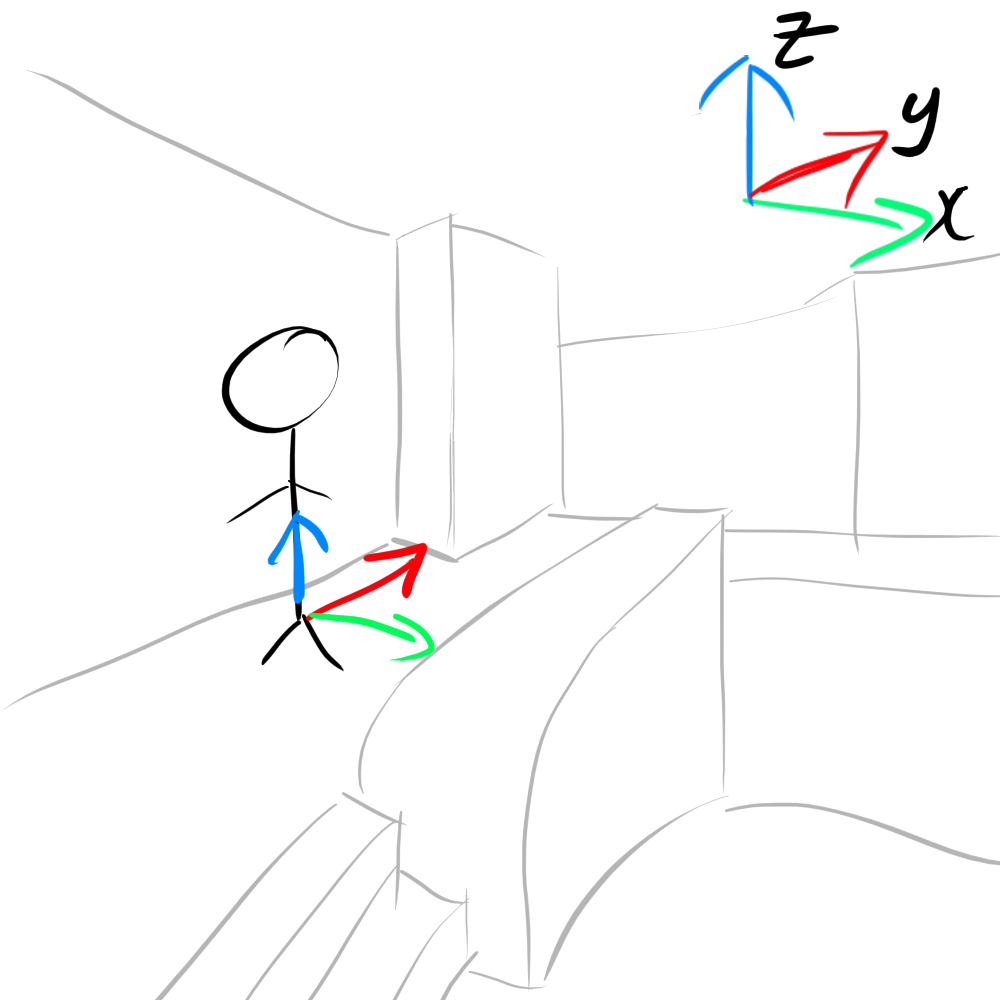
\includegraphics[width=0.9\linewidth]{assets/1coordinates.png}
        \caption{Coordinate system}
        \label{fig:1coordinates}
    \end{minipage}%
    \begin{minipage}{.5\textwidth}
        \centering
        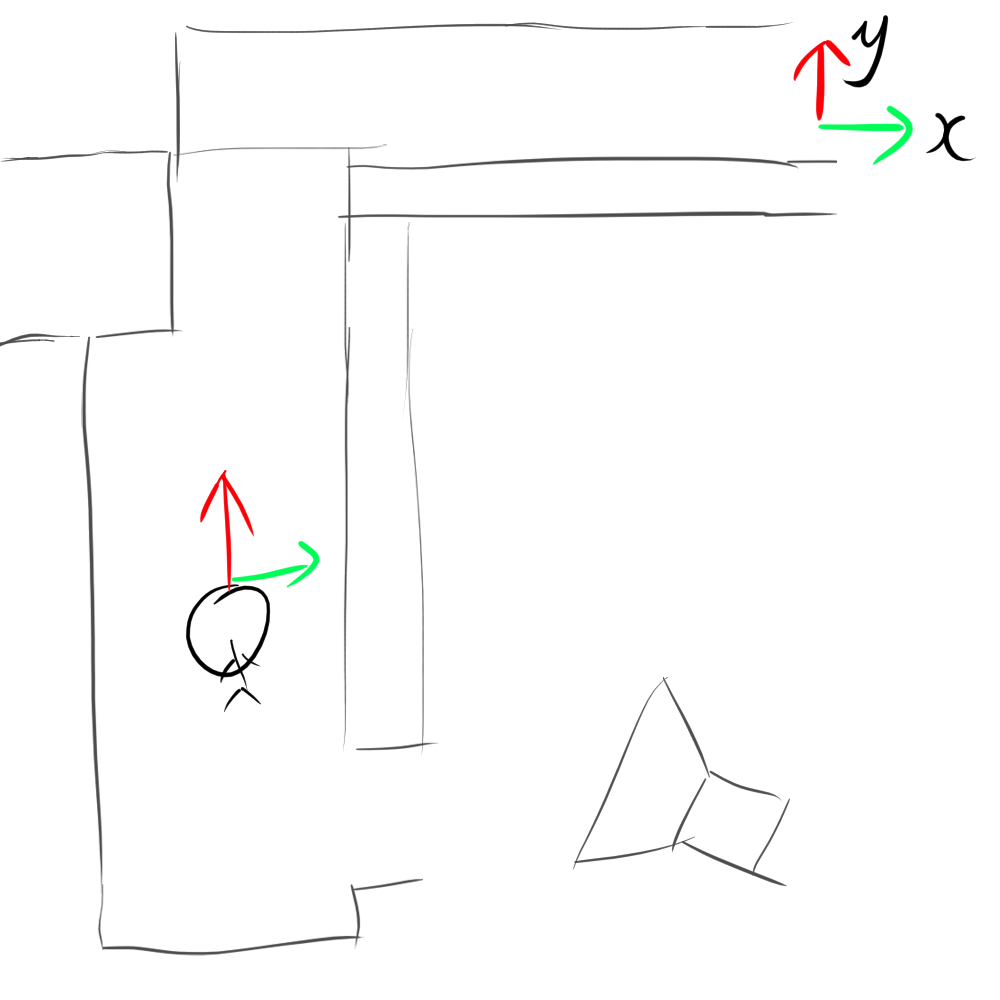
\includegraphics[width=0.9\linewidth]{assets/2coordinate_topdown.png}
        \caption{Top down view}
        \label{fig:2coordinates_topdown}
    \end{minipage}
\end{figure}


The problem is also top-down rotationally invariant. Let the z-axis denote the vertical axis, and the xy-axis to be the plane axis top down (see figure \ref{fig:1coordinates}, figure \ref{fig:2coordinates_topdown}).

\begin{figure}[H]
    \centering
    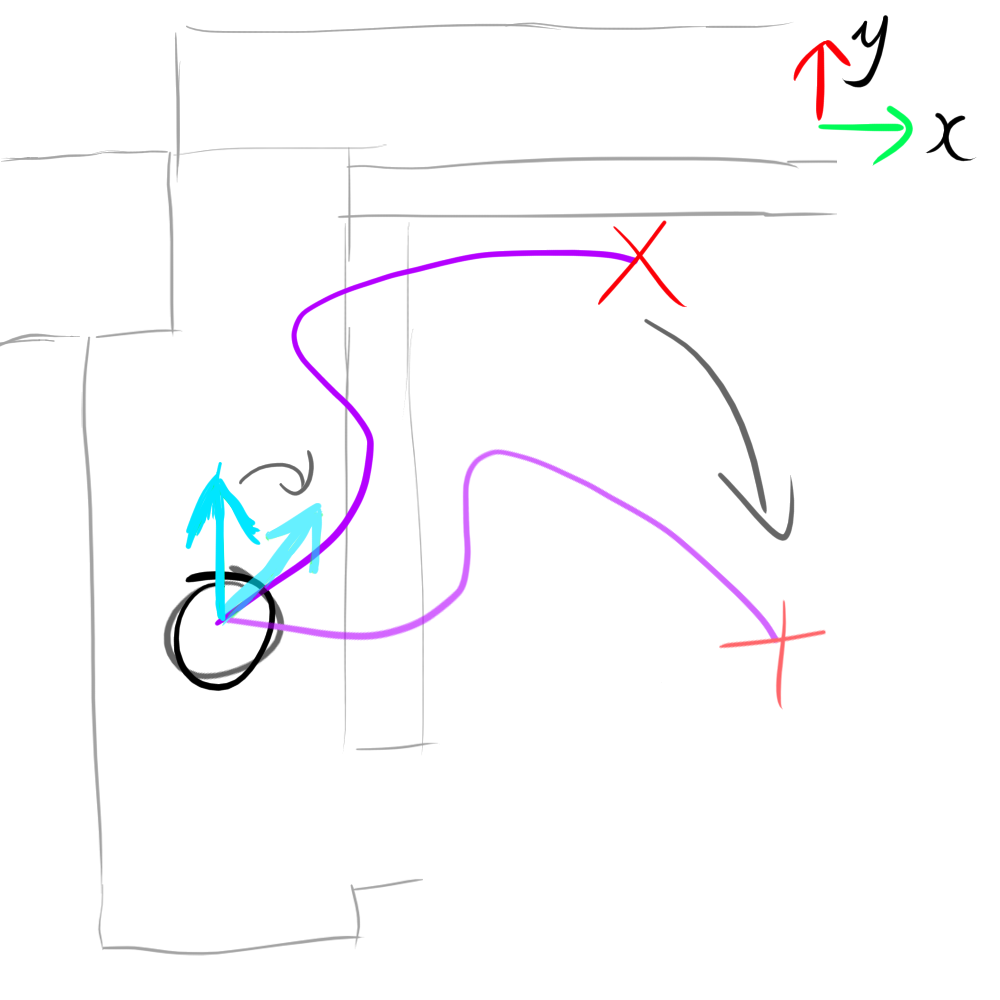
\includegraphics[width=0.4\textwidth]{assets/2turning.png}
    \caption{Rotational invariant (the player wishes to go rightwards)}
    \label{fig:2turning}
\end{figure}

In considering only the xy-axis, I realized that an optimal strategy does not depend on the angle of the initial velocity vector within the plane; It is always possible to rotate the initial velocity to rotate the direction of final displacement (see the blue vector and purple curve in figure \ref{fig:2turning}). This meant that the optimal initial velocity is rotational invariant, but I used the initial velocity in the y-axis for the sake of consistency between models:
\[
    \tv(0) = \tang{0, 250, 0}.
\]

Additionally, let the initial position of the player to be zero for ease of calculations:
\[
    \tp(0) = \tang{0, 0, 0}
\]

The z-axis initial velocity can be experimentally determined. This is because the player cannot accelerate in the z-axis during the jump, so the only vertical acceleration is initial\citefoot{chong_2022}. In fact, we will soon see that the z-axis can be pre-computed to reduce the dimensions of this problem.

\subsection{Straight line model}
With the key idea and boundary conditions in mind, I attempted a straight line strategy. This model has the player accelerate and move in a straight line, as mathematics has taught me that the shortest displacement between two points comes from a line, reducing the unnecessary displacements and maximizing total displacement. To achieve this, the player will accelerate along its initial velocity in the y-axis. Mathematically, this is equivalent to setting the directional vector to
\[
    \td(t) = \tang{0, 1}.
\]
Realistically, this will be equivalent to pressing down the move forward button and not moving the mouse that turns the player.
% do model!!
\begin{figure}[H]
    \centering
     \begin{minipage}{.5\textwidth}
        \centering
        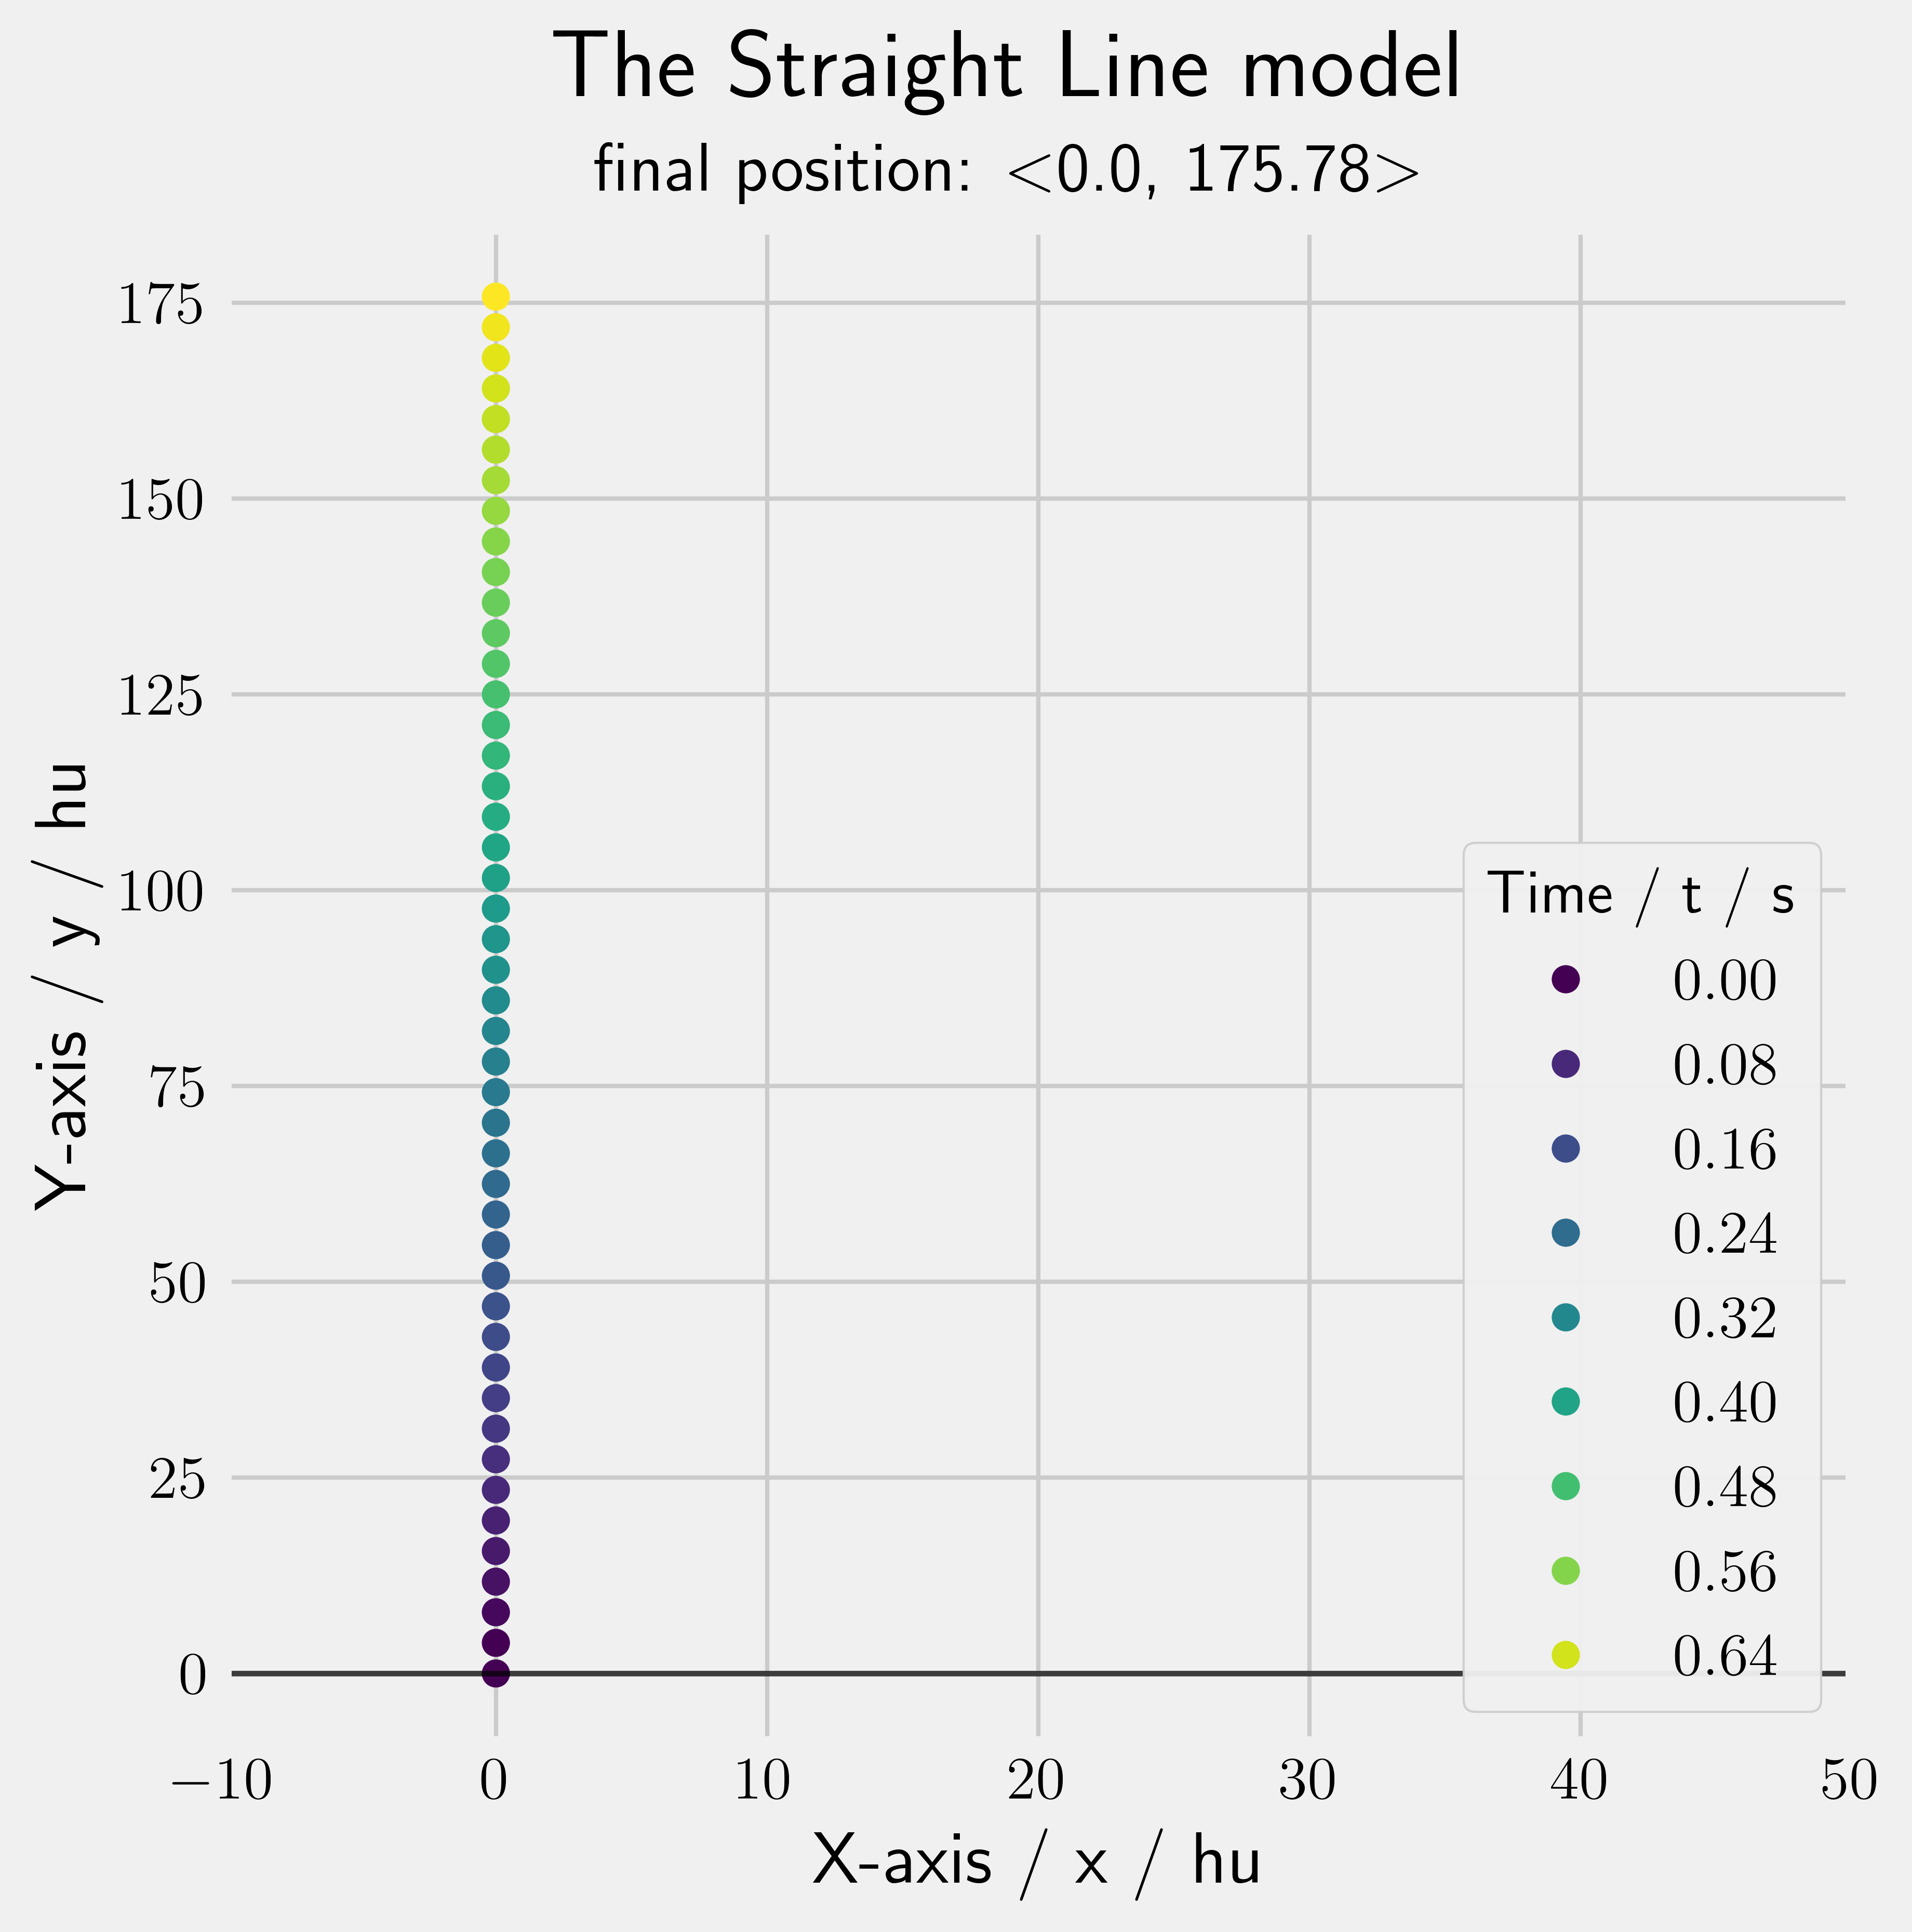
\includegraphics[width=0.9\linewidth]{assets/straight_constraint.png}
        \caption{Player movement}
        \label{fig:straight_constraint}
    \end{minipage}%
    \begin{minipage}{.5\textwidth}
        \centering
        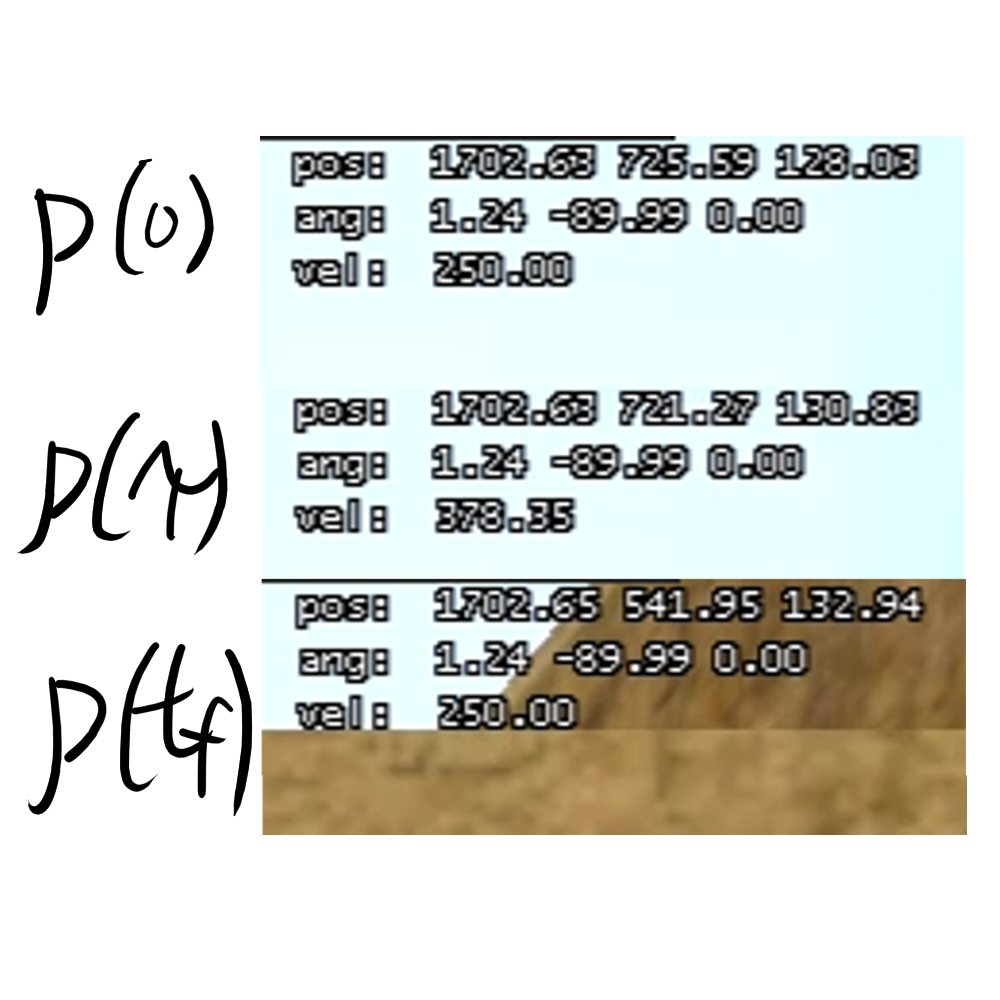
\includegraphics[width=0.9\linewidth]{assets/2straightjumping.png}
        \caption{Straight jumping}
        \label{fig:2straightjumping}
    \end{minipage}
\end{figure}

To test this model, I recorded myself jumping and performing the actions described above on a flat plane. Figure \ref{fig:straight_constraint} shows the estimation of the player's path using software\footnote{python37}\footnote{matplotlib}; Figure \ref{fig:2straightjumping} shows the coordinates of the player at the start of the jump $\tp(0)$, the first frame of the jump $\tp(\tau)$, and the end of the jump $\tp(t_f)$:
\begin{align}
 \tp(0) &= \tang{1702.63, 725.59, 128.03}, \quad \tmag{\tv(0)} = 250.00 \label{eq:2emp0}\\
 \tp(\tau) &= \tang{1702.63, 721.27, 130.83}, \quad \tmag{\tv(\tau)} = 378.35 \label{eq:2emp1}\\
 \tp(t_f) &= \tang{1702.65,541.95, 132.94}, \quad \tmag{\tv(t_f)} = 250.00 \label{eq:2emp2}.
\end{align}

\subsubsection{Straight line model analysis}
With the simple empirical data in Eq. \ref{eq:2emp0}, Eq. \ref{eq:2emp1}, and Eq. \ref{eq:2emp2}, not only can I analyze the straight line model, but it also allows me to model the vertical motion. However, I've noticed that the x,z-axis have changed after the jump. The $x$ change is likely the result of human errors in the player looking along the y-axis, but due to the rotational invariant discussed before, this is a non detrimental problem; but the z-axis changed after the jump --- I believe it to be the result of the ``bounciness'' as thelands from the jump\citefoot{bounce}, which can be ignored ($\Delta \tp_z = 0$).

The total displacement of this jump par our definition is the expression $d = \tmag{\tp(t_f) - \tp(0)}$, which is
\begin{align*}
    d &= \sqrt{(\tp_x(t_f) - \tp_x(0))^2 + (\tp_y(t_f) - \tp_y(0))^2 + (\tp_z(t_f) - \tp_z(0))^2}\\
    &= \sqrt{(1702.65-1702.63)^2 + (541.95-725.59)^2 + (0)^2}\\
    &\approx 183.64.
\end{align*}

Firstly notice the sudden change in the velocity of the player in first frame at time $\tau$. From this I deduced that the act of jumping is achieved by an impulse --- a sudden change in velocity --- upon the z-axis. With the assumption that no such impulses occurs in the xy-axis, and that the x,y-plane acceleration in the first frame is negligible, I found the size of the impulse using the Pythagorean Theorem\citefoot{Pythagoreantheorem} (figure \ref{fig:2verticalimpulse}).

\begin{align*}
    \tmag{\tv}^2 &= \tv_y^2 + \tv_z^2\\
    \tv_z &= \sqrt{\tmag{\tv}^2 - \tv_y^2}\\
    &= \sqrt{378.35^2 -250^2}\\
    &= 284.00.
\end{align*}

\begin{figure}[H]
    \centering
    %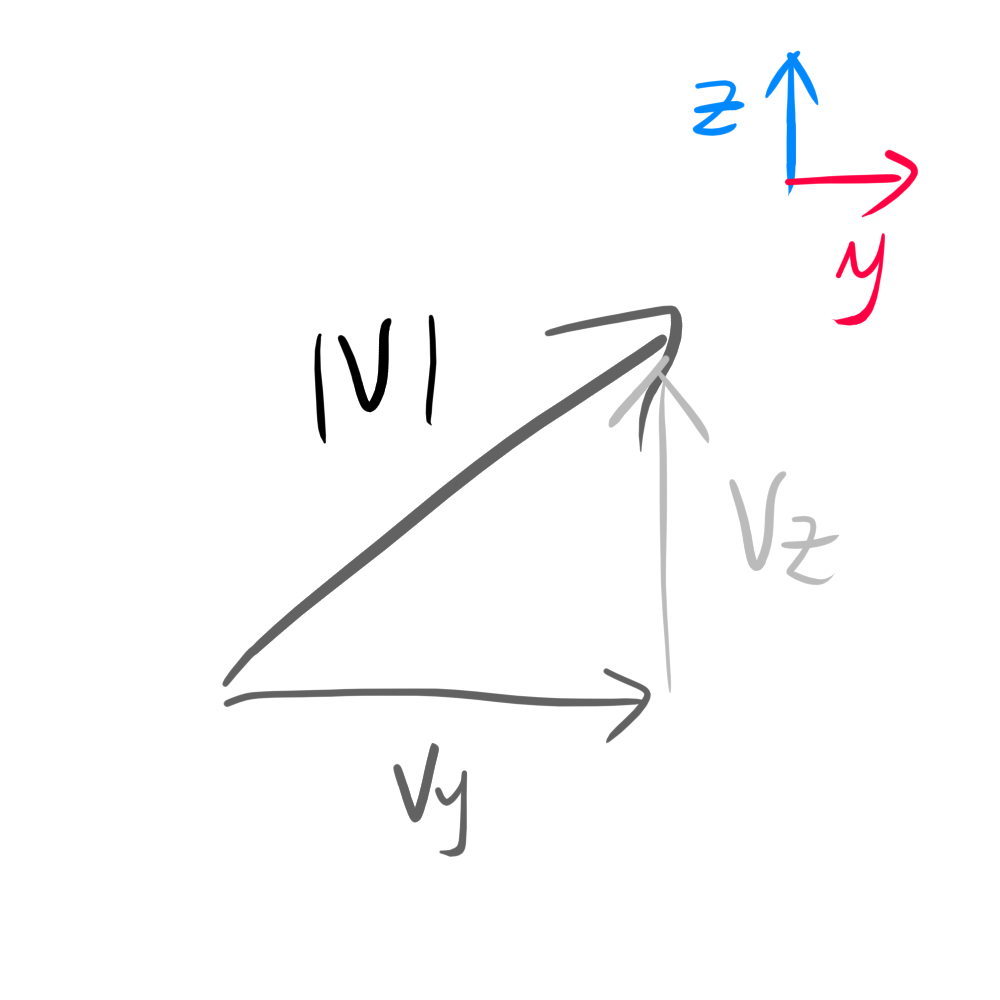
\includegraphics[width=0.37\textwidth,right]{assets/2verticalimpulse.png}
    \sized[0.4]{
        \tikzset{every picture/.style={line width=0.75pt}} %set default line width to 0.75pt

        \begin{tikzpicture}[x=0.75pt,y=0.75pt,yscale=-1,xscale=1]
            %uncomment if require: \path (0,236); %set diagram left start at 0, and has height of 236

            %Shape: Axis 2D [id:dp8024732250876303]
            \draw [color={rgb, 255:red, 0; green, 0; blue, 0 }  ,draw opacity=1 ] (418.43,41.53) -- (450,41.53)(421.59,10) -- (421.59,45.04) (443,36.53) -- (450,41.53) -- (443,46.53) (416.59,17) -- (421.59,10) -- (426.59,17)  ;
            %Straight Lines [id:da935697118906834]
            \draw    (290,150) -- (377.76,71.99) ;
            \draw [shift={(380,70)}, rotate = 138.37] [fill={rgb, 255:red, 0; green, 0; blue, 0 }  ][line width=0.08]  [draw opacity=0] (10.72,-5.15) -- (0,0) -- (10.72,5.15) -- (7.12,0) -- cycle    ;
            %Straight Lines [id:da37870943266053725]
            \draw    (290,150) -- (377,150) ;
            \draw [shift={(380,150)}, rotate = 180] [fill={rgb, 255:red, 0; green, 0; blue, 0 }  ][line width=0.08]  [draw opacity=0] (10.72,-5.15) -- (0,0) -- (10.72,5.15) -- (7.12,0) -- cycle    ;
            %Straight Lines [id:da23229694740869355]
            \draw [color={rgb, 255:red, 74; green, 144; blue, 226 }  ,draw opacity=1 ]   (380,150) -- (380,73) ;
            \draw [shift={(380,70)}, rotate = 90] [fill={rgb, 255:red, 74; green, 144; blue, 226 }  ,fill opacity=1 ][line width=0.08]  [draw opacity=0] (10.72,-5.15) -- (0,0) -- (10.72,5.15) -- (7.12,0) -- cycle    ;

            % Text Node
            \draw (429,42) node [anchor=north west][inner sep=0.75pt]  [xscale=1.25,yscale=1.25] [align=left] {{\fontfamily{pcr}\selectfont y}};
            % Text Node
            \draw (405,21) node [anchor=north west][inner sep=0.75pt]  [xscale=1.25,yscale=1.25] [align=left] {{\fontfamily{pcr}\selectfont z}};
            % Text Node
            \draw (321,160) node [anchor=north west][inner sep=0.75pt]  [color={rgb, 255:red, 80; green, 227; blue, 194 }  ,opacity=1 ,xscale=1.25,yscale=1.25] [align=left] {$\displaystyle \textcolor[rgb]{0,0,0}{v_{y}}$};
            % Text Node
            \draw (311,82) node [anchor=north west][inner sep=0.75pt]  [color={rgb, 255:red, 80; green, 227; blue, 194 }  ,opacity=1 ,xscale=1.25,yscale=1.25] [align=left] {$\displaystyle \textcolor[rgb]{0,0,0}{v}$};
            % Text Node
            \draw (392,102) node [anchor=north west][inner sep=0.75pt]  [color={rgb, 255:red, 80; green, 227; blue, 194 }  ,opacity=1 ,xscale=1.25,yscale=1.25] [align=left] {$\displaystyle \textcolor[rgb]{0.29,0.56,0.89}{v_{z}}$};


        \end{tikzpicture}
    }
    \caption{Jumping impulses}
    \label{fig:2verticalimpulse}
\end{figure}

For $\tau$ is small, I sat the player's initial vertical velocity to this number:
\[
    \tv_{z}(0) = 284.
\]

Secondly, by measuring the duration of the jump --- which I've done by counting the number of video frames of a $60\si{hz}$ video, or $44 \times \frac{1}{60} \approx 0.7333 \si{s}$ --- I was able to derive the average speed $\tv_{a}$ of the player:
\[
    \tv_{a} = \frac{183.71}{0.7333} \approx 250.42.
\]

Isn't that surprising? The average velocity does not differ from its initial value --- there is almost a zero net acceleration in the straight line model. The acceleration as a function of time $t$ and wishing direction $\td(t)$ could be zero in the xy-axis:
\[
    \ta(t, \td) = \tang{0, 0, ?}.
\]

I suspect a speed limit is in play here. This is bad in the optimization of jump displacement as it decreases the player's average velocity, which by the key idea, will limit the jump displacement. But it cannot be limiting the magnitude of velocity directly as I've personally achieved higher velocities while playing. One article explained this mechanic\citefoot{adrianb}. In short, the player's velocity $\tv$ is limited by its projection onto the directional vector $\td$.

\subsubsection{Projection speed limit}
\begin{figure}[H]
    \centering
    %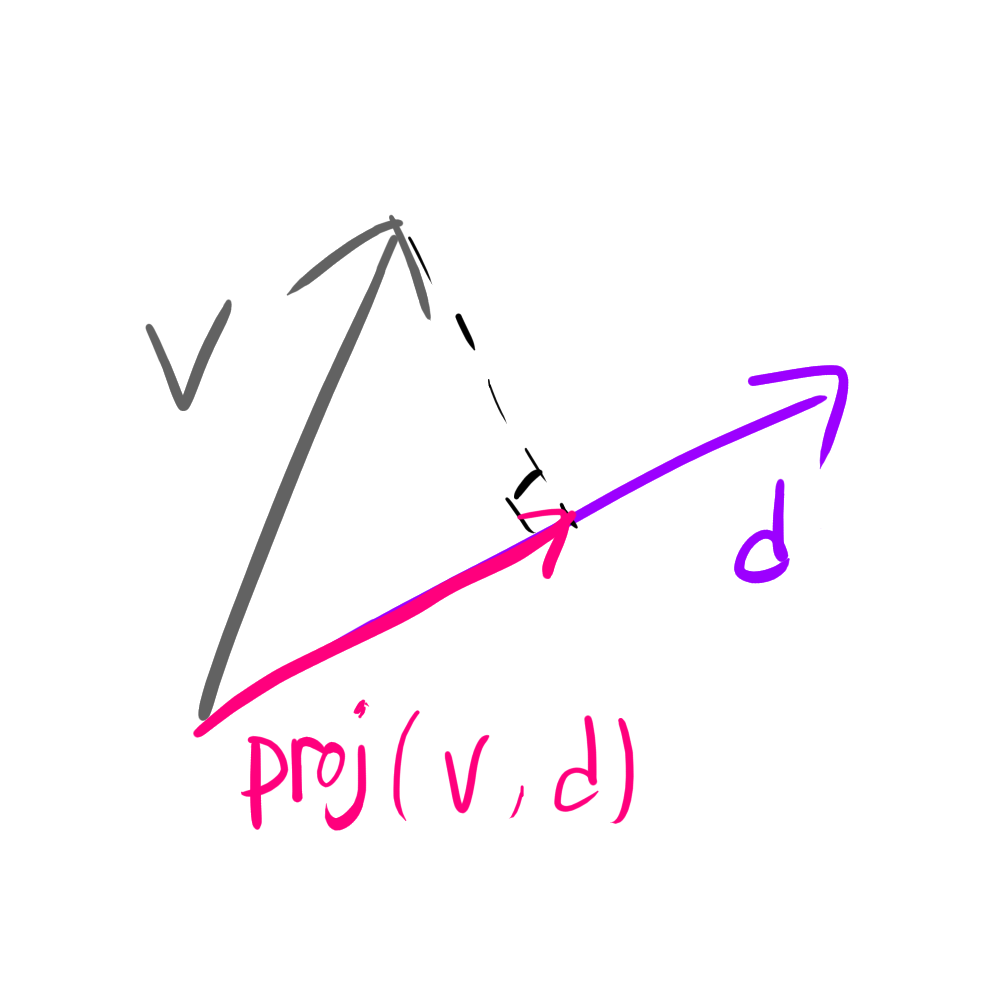
\includegraphics[width=0.37\textwidth,right]{assets/2proj.png}
    \sized[0.4]{


\tikzset{every picture/.style={line width=0.75pt}} %set default line width to 0.75pt

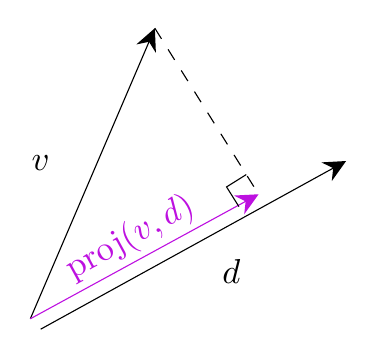
\begin{tikzpicture}[x=0.75pt,y=0.75pt,yscale=-1,xscale=1]
%uncomment if require: \path (0,201); %set diagram left start at 0, and has height of 201

%Straight Lines [id:da88922271648241]
\draw    (282,170) -- (340.82,32.76) ;
\draw [shift={(342,30)}, rotate = 113.2] [fill={rgb, 255:red, 0; green, 0; blue, 0 }  ][line width=0.08]  [draw opacity=0] (10.72,-5.15) -- (0,0) -- (10.72,5.15) -- (7.12,0) -- cycle    ;
%Straight Lines [id:da11348579225934163]
\draw [color={rgb, 255:red, 189; green, 16; blue, 224 }  ,draw opacity=1 ]   (282,170) -- (389.37,111.44) ;
\draw [shift={(392,110)}, rotate = 151.39] [fill={rgb, 255:red, 189; green, 16; blue, 224 }  ,fill opacity=1 ][line width=0.08]  [draw opacity=0] (10.72,-5.15) -- (0,0) -- (10.72,5.15) -- (7.12,0) -- cycle    ;
%Straight Lines [id:da5945932118539943]
\draw  [dash pattern={on 4.5pt off 4.5pt}]  (342,30) -- (392,110) ;
%Shape: Right Angle [id:dp9723060706204649]
\draw   (382.51,115.95) -- (376.55,106.46) -- (386.05,100.51) ;
%Straight Lines [id:da7502223575804331]
\draw    (287,175) -- (431.52,95.43) ;
\draw [shift={(434.15,93.98)}, rotate = 151.16] [fill={rgb, 255:red, 0; green, 0; blue, 0 }  ][line width=0.08]  [draw opacity=0] (10.72,-5.15) -- (0,0) -- (10.72,5.15) -- (7.12,0) -- cycle    ;

% Text Node
\draw (294.24,139.42) node [anchor=north west][inner sep=0.75pt]  [color={rgb, 255:red, 189; green, 16; blue, 224 }  ,opacity=1 ,rotate=-331.37,xscale=1.25,yscale=1.25] [align=left] {proj$\displaystyle ( v,d)$};
% Text Node
\draw (281,90) node [anchor=north west][inner sep=0.75pt]  [xscale=1.25,yscale=1.25] [align=left] {$\displaystyle v$};
% Text Node
\draw (373,140) node [anchor=north west][inner sep=0.75pt]  [xscale=1.25,yscale=1.25] [align=left] {$\displaystyle d$};


\end{tikzpicture}

    }
    \caption{Projection limiting}
    \label{fig:2proj}
\end{figure}

A vector's projection onto another is a way to say how much of the vector is pointing in the direction of another, in the form of a number. Denoted by $\text{proj}(\tv, \td)$, the projection of the player's velocity vector onto its direction vector is the side of the triangle formed by a perpendicular line from $\tv$ to $\td$ (figure \ref{fig:2proj}). This can be defined using a dot product:
\[
    \text{proj}(\tv, \td) = \frac{\tv \cdot \td}{\tmag{\td}}.
\]

Also, because the z-component of $\td$ is always zero, the projection is simply the 2-vector dot product between $\tv$ and $\td$.
\begin{align*}
    \text{proj}(\tv, \td) &= \tv \cdot \td\\
    &= \tv_x \td_x + \tv_y \td_y + \tv_z \td_z\\
    &= \tv_x \td_x + \tv_y \td_y.
\end{align*}

Crucially, this projection vector is limited by an engine constant $L$ set to $250$ (all engines constants\citefoot{wei_2022}). If the projection exceeds $L$, acceleration will be zero; else, acceleration is a constant in the direction of $\td$ equal to $LA\tau$ in the discrete sense, and $LA$ in the continuous approximation --- with $A$ being $10$, another engine constant. The player's planer acceleration function can therefore be defined piecewisely as:
\begin{figure}[H]
    \centering
    \[
        \ta_{xy}(t) = \begin{cases}
            LA \td(t) & \text{proj}(\tv, \td) < L\\
            0 & \text{proj}(\tv, \td) \geq L
        \end{cases}
    \]
        \caption{Player planer acceleration function}
    \label{eq:playeracceleration}

\end{figure}

To maximize displacement, we would want the first condition of equation \ref{eq:playeracceleration} to be true for as long as possible. Yet in the context of my straight line model, it is simple to see that the first condition is never true, for
\begin{align*}
    \text{proj}(\tv, \td) &= \tv_x \td_x + \tv_y \td_y\\
    &= \tv_x \times 0 + \tv_y \times 1\\
    &= \tv_y,\\
    \because \quad \tv_{y}(0) &= 250 = L\\
    \text{proj}(\tv, \td) &= L\\
    \therefore  \quad \ta(t) &= 0.
\end{align*}

My acceleration model has confirmed my hypothesis that the player is not accelerating in the xy-axis during the jump. By the key idea, this will reduce the average velocity and in turn, reduces the total displacement of the jump.

\subsubsection{Continuous modeling approximation}
But before I try some other models, let's first evaluate the accuracy of the continuous approximation using this simplistic model. The same article\citefoot{adrianb} reveals an engine constant z-axis acceleration $g$ equal to $800$, and I thought of this as an opportunity to test my continuous approximation by comparing my calculated value with the real value.

The objective is to solve the differential equations of motion for the player. For the xy-axis acceleration of the player is zero, and let $g$ be the signed z-axis acceleration:
\[
    \ta = \tang{0, 0, g},
\]
the velocity as defined in Eq. \ref{eq:1de1} is the integral of acceleration:
\begin{align*}
    \tv(t) &= \int \ta(t) \, dt\\
    &= \tpars{0}{0}{gt} + \tv(0)\\
    &= \tpars{0}{0}{gt} + \tpars{0}{250}{284}\\
    &= \tpars{0}{250}{gt + 284}.
\end{align*}

Continuing, the player position is the integral of velocity as shown in Eq. \ref{eq:1de2}:
\begin{align*}
    \tp(t) &= \int \tv(t) \, dt\\
    &= \tpars{0}{250t}{\frac{1}{2}gt^2 + 284t} + \tp(0)\\
    &= \tpars{0}{250t}{\frac{1}{2}gt^2 + 284t}
\end{align*}
shows that the the y-axis displacement is $250t$. Because the actual displacement is $\approx 183.64$, this means that the jump duration $t_f$ is
\[
    t_f = \frac{183.64}{250} \approx 0.735 \si{s}.
\]
Since the z-axis displacement is zero, the gravitational acceleration $g$ is calculated to be
\begin{align*}
    \tp_{z}(t_f) &= \frac{1}{2}gt_f^2 + 284t_f = 0\\
    g &= - 2 \times \frac{284t_f}{t_f^2}\\
    &= -\frac{568}{t_f}\\
    &\approx -772.79.
\end{align*}

Comparing to the actual value of $g$, $772.79$ is not far off --- the relative error of $\frac{800 - 772.79}{800} \approx 3.4\%$ is small enough for an approximation. Therefore it is justified that I can continuously use the continuous approximations, to which I will.

Furthermore, the lack of correlation between the z-axis on the xy-axis and vice versa ($\tp_z(t_f)$ doesn't depend on $\td$) means that no changes in the xy-axis can change the z-axis --- the jump duration $t_f$ is constant. Therefore all subsequent models will be uniquely identified by their planer $\td(t)$ functions.

\subsection{Skilled player's model}
A better strategy would be the player accelerating not directly along their velocity, but rather at an angle to their velocity. Personally I've been told by numerous skilled players that you need to move your mouse slowly to the right --- meaning rotating the vector $\td$ over time --- to get higher speed and distance. Now I can test this theory.

Currently, any strategy is uniquely defined by the player's direction function $\td(t)$ as a real 2-vector. This model will point $\td(t)$ towards the y-axis at $t=0$, and rotate clockwise over time. This reminded me of a unit circle with the xy-axis switched, creating
\[
    \td(t) = \tang{\sin(t), \cos(t)}.
\]

Additionally, I can encode the rate of rotation by scaling the inner $t$ in the two trig functions by the same factor $w$. Therefore, the player direction function $\td(t)$ as recommended by skilled players is
\[
    \td(t) = \tang{\sin(wt), \cos(wt)}.
\]
This definition will always have unit magnitude:
\begin{align*}
    \tmag{\td(t)} &= \sqrt{\td_x(t)^2 + \td_y(t)^2}\\
    &= \sqrt{\sin^2(wt) + \cos^2(wt)}\\
    &= \sqrt{1}\\
    &= 1.
\end{align*}

My task is to find the constant $w$ that maximizes displacement.

%The plan is to solve the xy-axis differential equation into a positional function $\tp(t)$, then explicitly writing the speed limit as an inequality constraint, and finally selecting the constant $w$ that (hopefully) satisfies the constraint and maximizes the displacement.

\subsubsection{Displacement equation}
The plan is to solve the xy-axis differential equation into a positional function $\tp(t)$. The key idea suggests that I should maximize the velocity, and as explained in the subsection before, this meant that player acceleration $\ta(t)$ is to be maximized by fulfilling the inequality projection in equation \ref{eq:playeracceleration}. When this inequality is held,
\[
    \ta(t) = LA\td(t).
\]

Let $k=LA$. Notice that the velocity is the integral of acceleration,
\begin{align*}
    \tv(t) &= \int \ta(t) \, dt\\
    &= \int k \tpar{\sin(wt)}{\cos(wt)} \, dt\\
    &= \frac{k}{w} \tpar{-\cos(wt)}{\sin(wt)} + c_v,\\
    \tv(0) &= \frac{k}{w} \tpar{-\cos(0)}{\sin(0)} + c_v\\
    c_v &= \frac{k}{w} \tpar{1}{0} + \tpar{\tv_x(0)}{\tv_y(0)}.
\end{align*}

And the position is the integral of velocity,
\begin{align*}
    \tp(t) &= \int \tv \, dt\\
    &= \int \frac{k}{w} \tpar{-\cos(wt)}{\sin(wt)} + \frac{k}{w}\tpar{1}{0} + \tpar{\tv_x(0)}{\tv_y(0)} \, dt\\
    &= \frac{-k}{w^2} \tpar{\sin(wt)}{\cos(wt)} + \frac{k}{w}\tpar{t}{0}  + t\tpar{\tv_x(0)}{\tv_y(0)} + c.
\end{align*}

To find the integration constant $c$, consider the x-axis displacement function
\begin{align*}
    \tp_x(t) &= \frac{-k}{w^2} \sin(wt) + t\tv_x(0) + t\tv_x(0) + c_x = 0\\
    c_x &= 0,
\end{align*}
and the y-axis displacement function
\begin{align*}
    \tp_y(t) &= \frac{-k}{w^2} \cos(wt) + t\tv_y(0) + c_y = 0\\
    c_y &= \frac{k}{w^2}.
\end{align*}

Using the Pythagorean Theorem, the magnitude of the player's displacement using this model after a jump at $t=t_f$ is:
\begin{figure}[H]
    \centering
    \begin{align*}
        \tmag{\tp(t_f) - \tp(0)} &= \sqrt{\tp_x(t_f)^2 + \tp_y(t_f)^2}\\
        &= \sqrt{\left(\frac{-k}{w^2}\sin(wt_f) + t_f\frac{k}{w} \right)^2 + \left( \frac{-k}{w^2}\cos(wt_f) + 250t_f + \frac{k}{w^2} \right)^2}
    \end{align*}
    \caption{Skilled Displacement}
    \label{eq:2skilled_displacement}

\end{figure}

\begin{figure}[H]
    \centering
    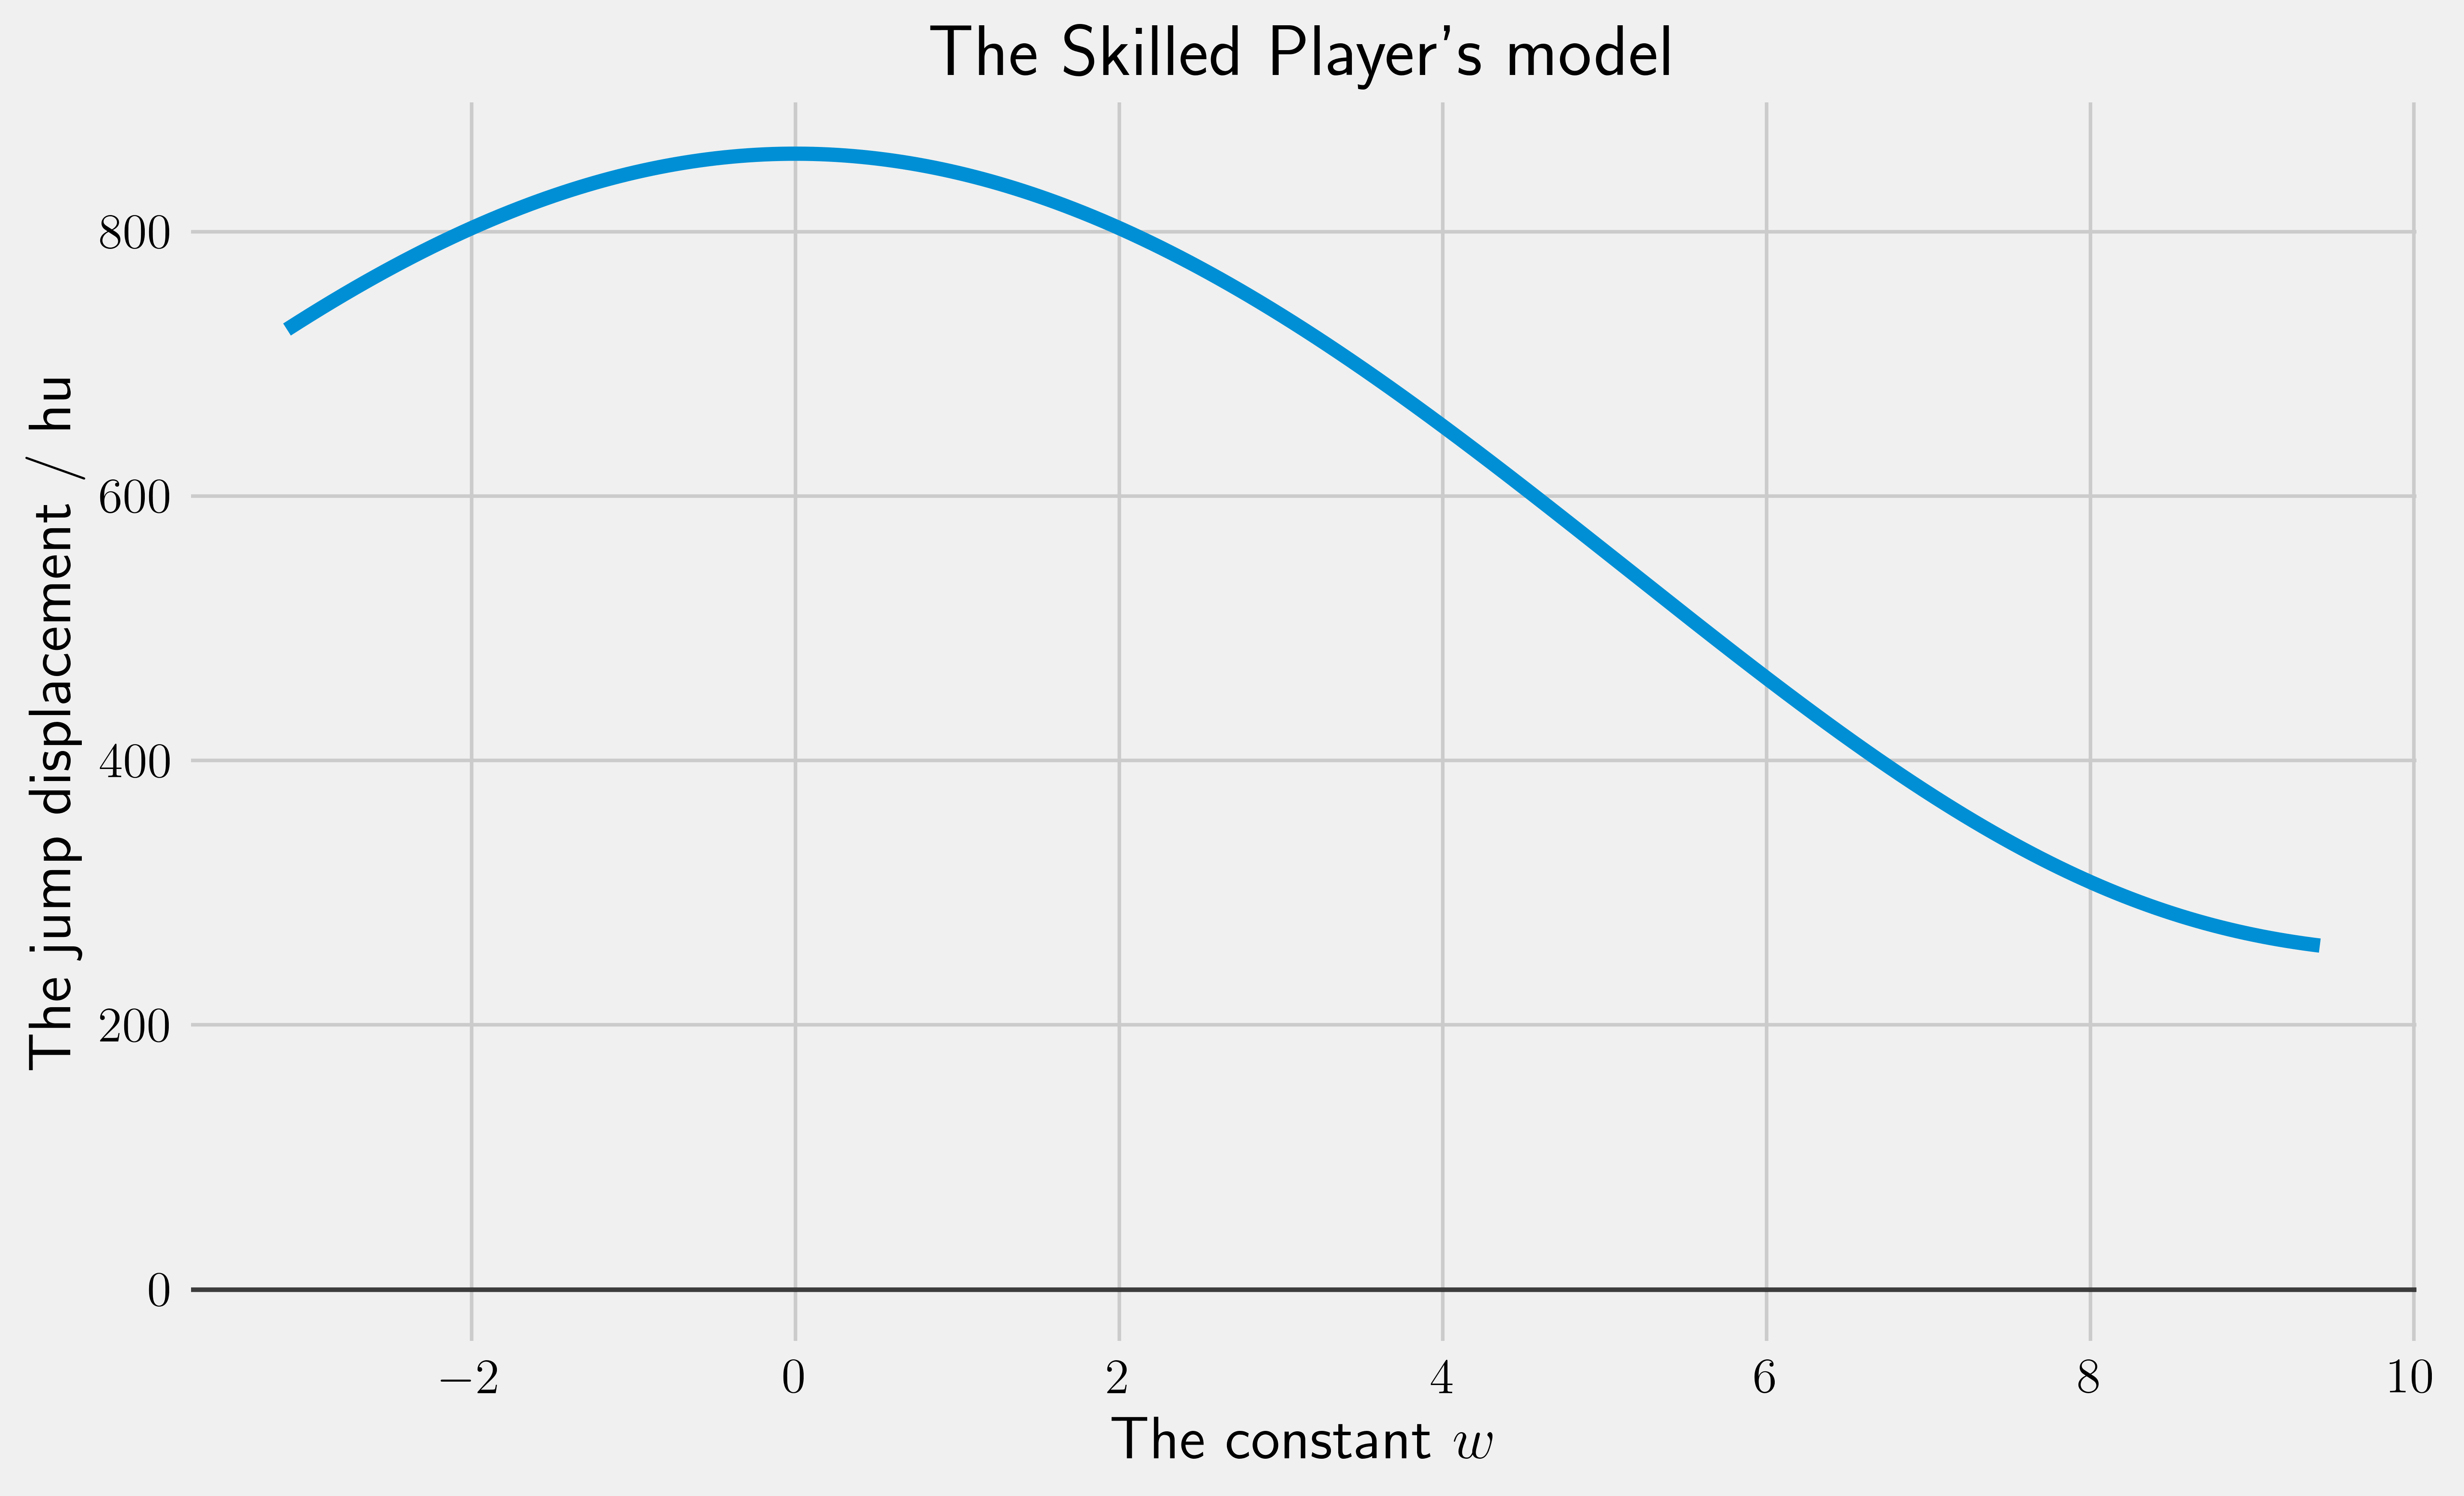
\includegraphics[width=0.85\textwidth]{assets/skilled_displacement.png}
    \caption{}
    \label{fig:skilled_displacement}

\end{figure}
The graph of equation \ref{eq:2skilled_displacement} shown in figure \ref{fig:skilled_displacement} is symmetrical along the y-axis due to the rotational invarance. Quantitatively, this unrestricted function peeks when $w=0$ when the strategy collapses to my straight line model. As the turning speed $w$ increases, the ideal displacement decreases and levels near $w=10$: I guess that a spinning player does not contribute much to jumping far. Therefore we need to choose the smallest $w$ possible to maximize potential jump displacement.

\subsubsection{Restriction equation}
In addition to finding the unrestricted displacement of the strategy for all constants $w$, we also need check if they satisfy the assumption of unrestricted acceleration at all times. Ideally there should be a value of $w$ that always fits this constraint, but the smallest ``error'' from the ideal is always a backup option.

By assumption of the restricted equation, the constraint
\[
    \text{proj}(\tv, \td) < L
\]
must be held for the duration of the jump. Expanding and organizing this inequality yields
\begin{align*}
    L &> \text{proj}(\tv, \td)\\
    &> \tv_x \td_x + \tv_y \td_y\\
    &> \left(-\frac{k}{w} \cos(wt) + \frac{k}{w}\right) \sin(wt) + \left(\frac{k}{w} \sin(wt) + 250\right) \cos(wt),\\
    0 &> \left(-\frac{k}{w} \cos(wt) + \frac{k}{w}\right) \sin(wt) + \left(\frac{k}{w} \sin(wt) + 250\right) \cos(wt) - 250
\end{align*}

To find the value of the constant $w$ that best fulfills this inequality would need a quantitative measure on how well this inequality is held through the jump. Ideally the function should only include the failures of fulfilling the inequality, but to be explained in the more advanced models --- that the projection RHS should be as close to zero as possible for high speeds --- I chose an integral from $t=0$ to $t=t_f$ on the absolute values of the RHS, denoted as the error of a model. This uses absolute function $|x|$ defined by
\[
 |x| = \begin{cases}
         x & x \geq 0\\
         -x & x < 0
        \end{cases}
\]
as to make all errors positive. Therefore the error function $R(w)$ for each constant $w$ is:
\begin{figure}[H]
 \centering
 \[
  R(w) = \int_0^{t_f} \left|\left(-\frac{k}{w} \cos(wt) + \frac{k}{w}\right) \sin(wt) + \left(\frac{k}{w} \sin(wt) + 250\right) \cos(wt) - 250\right| \, dt
 \]
 \caption{The error function}
 \label{eq:2error}
\end{figure}


\begin{figure}[H]
 \centering
 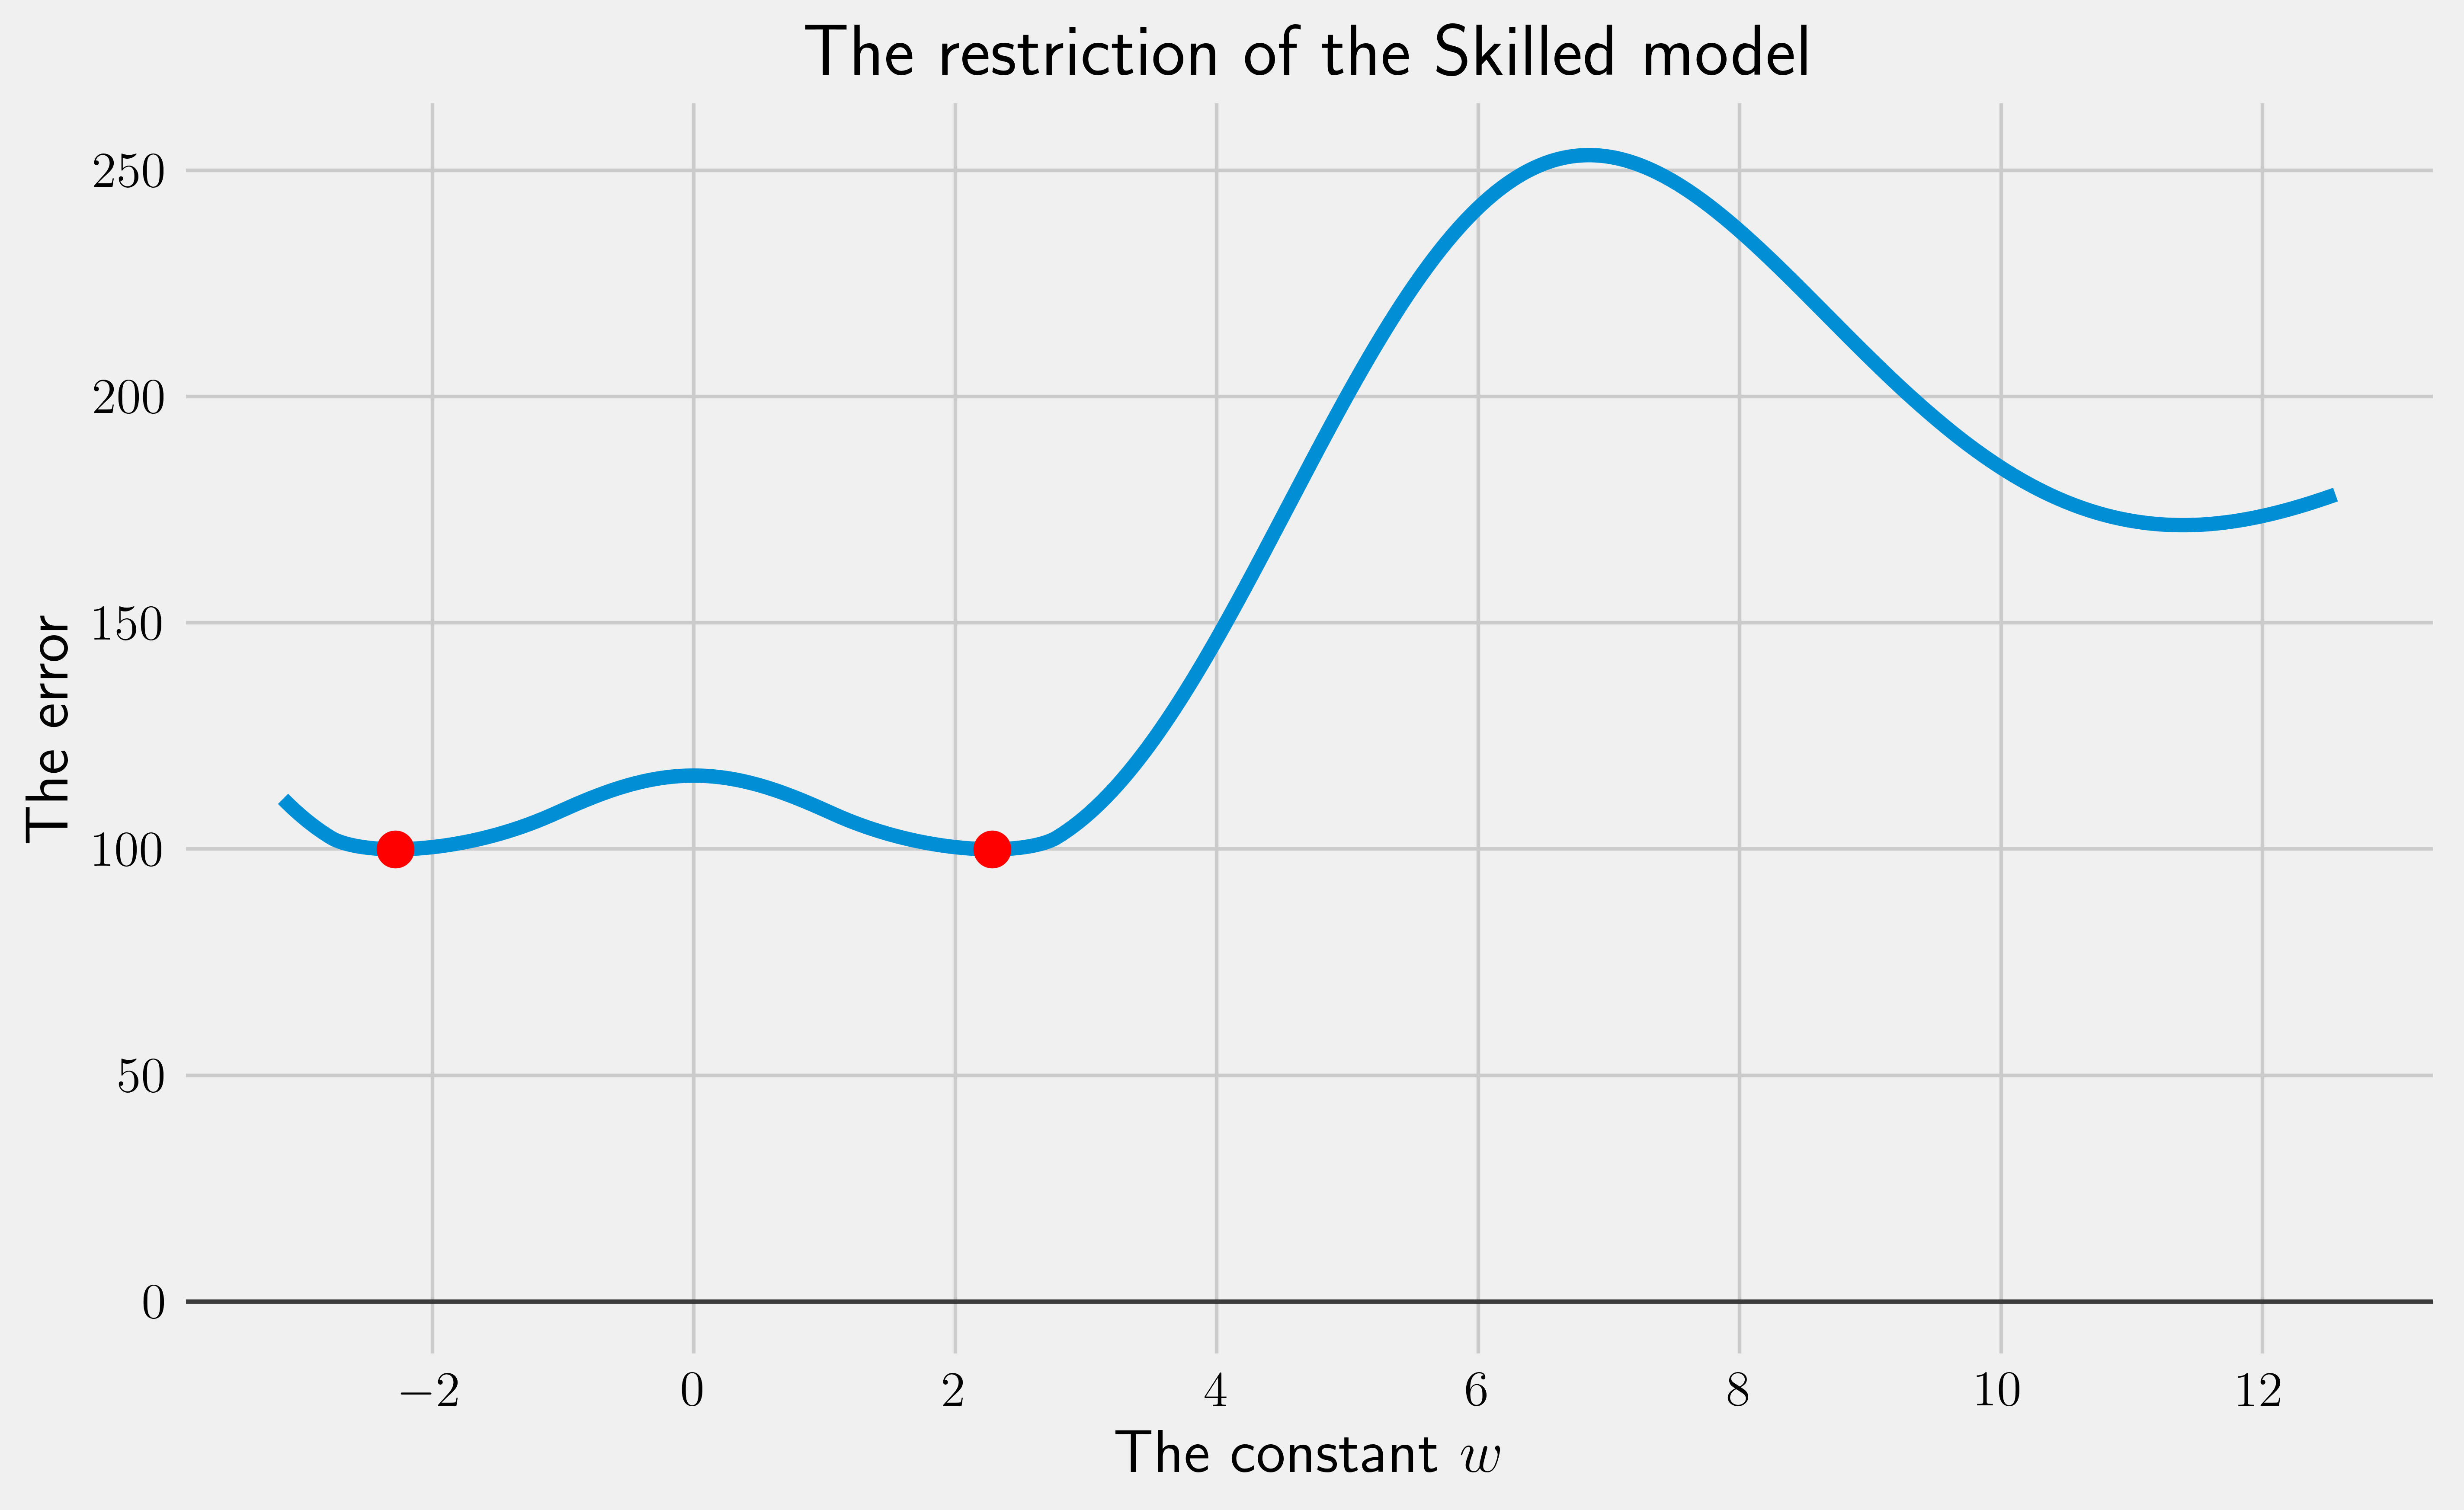
\includegraphics[width=0.85\textwidth]{assets/restriction_equation.png}
 \caption{}
 \label{fig:2error}
\end{figure}
% TODO: if needed, show the two red dots and choose the smallest one
Figure \ref{fig:2error} shows the graph of the error function in equation \ref{eq:2error}. While it may be possible to find the minimum of the error function using calculus, the steps are too complex and a numerical solution is taken instead shown by the red dot in the graph.

My program shows that the red dot is at coordinate
\[
    \tang{4.2884, 184.4228},
\]
meaning that the error function is at the smallest when $w=4.2884$. I can therefore conclude that the skilled player's model is defined by
\[
    \td(t) = \tang{\sin(4.2884t), \cos(4.2884t)},
\]
indicating a relatively fast rate of turning of a period $\frac{2\pi}{4.2884} = 1.4652\si{s}$.

\begin{figure}[H]
    \centering
    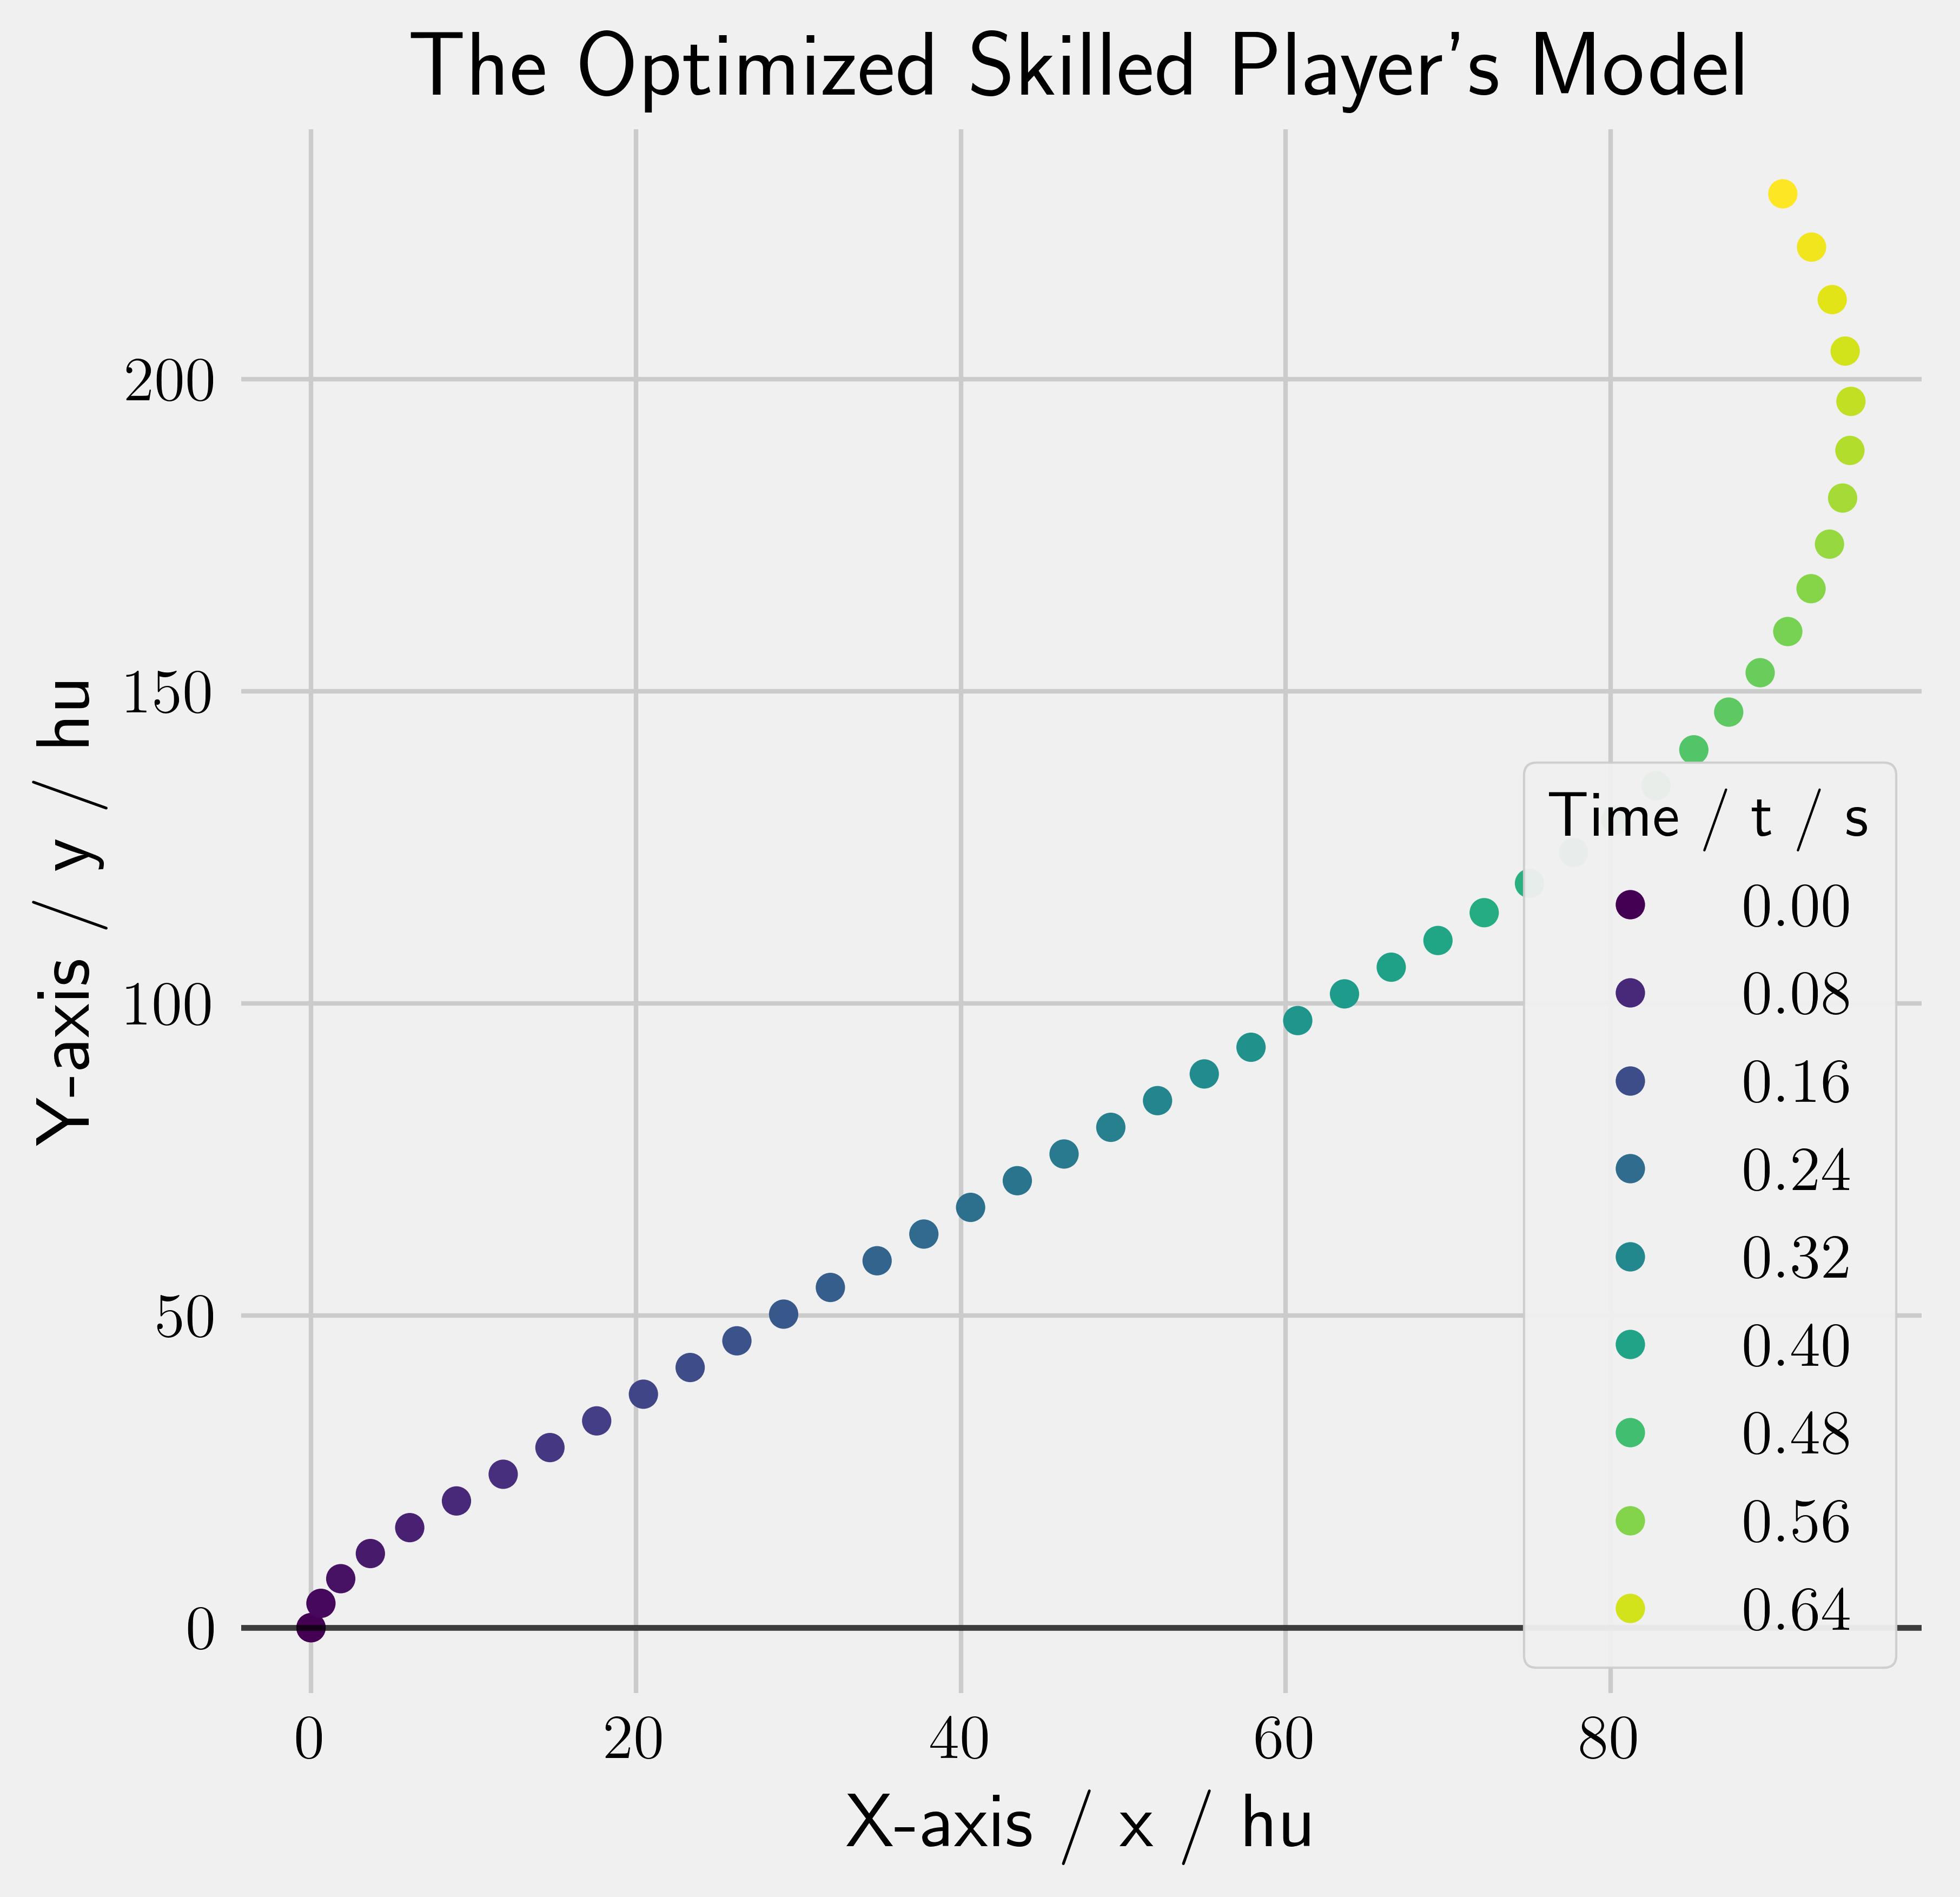
\includegraphics[width=0.55\textwidth]{assets/skilled_player.png}
    \caption{Skilled Player's Model}
    \label{fig:skilled_player}
\end{figure}


When unrestricted, there should be a displacement of $627.35$ using figure \ref{fig:skilled_displacement}. But I suspect error $184.4228$ had decreased the displacement by quite an amount. Figure \ref{fig:skilled_player} shows the actual path of the player when simulated in game; this is in combination with a correctly estimated lower displacement of $254.19$ units.
\begin{align*}
    \tp(t_f) &= \tang{88.3021, 238.3556}\\
    \tmag{\tp(t_f)} &\approx 254.19
\end{align*}

The skilled player's model does indeed produce a higher displacement ($254.19$) than the straight line model ($183.64$). Not only does this confirm the theory from these skilled people, but the large error of the even optimized model could indicate further possible optimizations when I look at the problem discretely.
